\section{Entwicklung} % (fold)
\label{sec:entwicklung}
	Dieses Kapitel soll den Entwicklungsprozess konkretisieren und den Optimierungsprozess einer Webanwendung aufzeigen. Es soll erläutern, welche Fragen sich stellten und welche Antworten darauf gefunden wurden. Wie bestimmte Probleme gelöst wurden. Welche Tools und Hilfsmittel zur verwendung kamen. Dies soll ein Bewusstsein dafür schaffen, was möglich ist und wie eine technische Umsetzung aussehen kann. 
	
	\subsection{Tools}
	\label{sub:tools}
		Dies ist eine Auflistung an Tools und nützlichen Seiten, die entweder im Projekt verwendet, oder die für Wertvoll befunden wurden und deshalb hier ihren Platz finden, damit jeder für sich entscheiden kann, ob der Einsatz davon sinnvoll sein könnte.

		\subsubsection{Google Chrome Developer Tool} % (fold)
		\label{ssub:google_chrome_developertool}
			Dieses Tool ist über die Taste F12 im Chrome Browser zu finden. Nützliche Features sind: 

			\begin{itemize}
				\item \texttt{Device Emulation} \footnote{Bei geöffnetem Tool (F12): strg + shift + M oder klick auf das Smartphone Symbol}: Damit lassen sich verschiedene Devices wie Smartphones, Ipad oder verschiedene Desktopauflösungen simulieren. Auch das Touch verhalten wird Simuliert.
				\item In der Device Emulation lässt sich auch die Netzwerkgeschwindigkeit simulieren. Dies ist allerdings nur eine Simulation und kann unter wahren Bedingungen stark abweichen.
				\item Netzwerk: Hier lässt sich das Wasserfallmodell nachvollziehen. Auch lässt sich hier das Caching des Browsers abschalten, wärend das Developer Tool geöffnet ist.
				\item Audits: Unter diesem Reiter bekommt man erste Informationen, welche Verbesserungen es für diese Seite aus dem Gesichtspunkt der Performance ergeben. So wird zum Beispiel aufgezeigt, wie viele CSS Selektoren auf dieser Seite gar keine verwendung finden (gerade bei CSS-Frameworks wie Bootstrap kann es sein, dass rund 90\% der Selektoren keine Verwendung haben)
			\end{itemize}
		% subsubsection google_chrome_developertool (end)

		\subsubsection{Google Pagespeed Insight} % (fold)
		\label{ssub:google_pagespeed_insight}
			Pagespeed Insight ist ein Analysetool für Webanwendungen. Per URL Eingabe wird die Anwendung Aufgerufen und gegen die "`Best Practices"' von Google getestet: \footnote{ \url{http://tinyurl.com/nvxksks} }. Dabei wird ein Rating von 1 (schlecht) bis 100 (gut) vergeben. Mobile und Desktop Version werden voneinander unabhängig bewertet. Findet das Tool verstöße gegen die \texttt{best practices}, so gibt es Hilfestellungen wie zum Beispiel weiterführende Links oder Hinweise zur Behebung des Problems. Für die Verbesserung der Perfomance ist dieses Tool eines der besten Anlaufziele, um einen Überblick zu bekommen wo sich die Probleme befinden. Pagespeed Insight gibt es auch als Plugin für das Google Chrome Developer Tool.\footnote{Plugin - Pagespeed Insight: \url{http://tinyurl.com/mv8fcx8}}
		
		% subsubsection google_pagespeed_insight (end)

		\subsubsection{Google Closure Compiler} % (fold)
		\label{ssub:closure_compiler}
			Ein simples Tool von Google\footnote{\url{http://closure-compiler.appspot.com/}}, mit der Aufgabe Javascript zu verkleinern. Dieser Vorgang nennt sich auch "`minify"' und ist auch für HTML und CSS möglich. Ein Beispiel:

			\begin{lstlisting}[captionpos=t, caption=Input, label=lst:minifyInput]
			/**
			 * urlEncodes an object to send it via post
			 * @param  {Object} object Object with key value pairs
			 * @return {String}        string in format key=value&foo=bar
			 */
			var urlEncode = function (object) {
			  var encodedString = '';
			  for (var prop in object) {
			    if (object.hasOwnProperty(prop)) {
			      if (encodedString.length > 0) {
			          encodedString += '&';
			      }
			      encodedString += encodeURI(prop + '=' + object[prop]);
			    }
			  }
			  return encodedString;
			};
			\end{lstlisting}

			Wird zu:

			\begin{lstlisting}[captionpos=t, caption=Output, label=lst:minifyOutput, breaklines=false]
			var urlEncode=function(c){var a="",b;for(b in c)c.hasOwnProperty(b)&&
			(0<a.length&&(a+="&"),a+=encodeURI(b+"="+c[b]));return a};
			\end{lstlisting}

			Wie zu sehen ist, werden nicht nur alle Kommentare, Leerzeichen und Zeilenumbrüche entfernt, sondern auch Variablennamen werden auf 1 Zeichen reduziert um weitere bytes zu sparen. Die Funktionalität bleibt dabei gewährleistet. Dieser Vorgang ist auch unter dem Namen "`uglify"' bekannt.
		
		% subsubsection closure_compiler (end)

		\subsubsection{Webpagetest} % (fold)
		\label{ssub:webpagetest}
			\url{Webpagetest.org} ist das wohl umfangreichst und beste Website-Analysetool das im Internet zu finden ist. Es ist ein kostenloser Service der hauptsächlich von Patrick Meenan entwickelt wurde. Das Tool ist leicht zu bedienen aber schwer zu beherschen ("`easy to use, hard to master"') und es gibt zahllose Einstellungen und undokumentierte Funktionen auf die man nur in Vorträgen oder Foren stoßt. Es gibt auch ein Buch, dass sich nur mit diesem Tool beschäftigt, beim Verlag \texttt{O'Reilly}.\footnote{Buch - Using WebPagetest: \url{http://shop.oreilly.com/product/0636920033592.do}}.	Die Features für Webpagetest sind vielseitig:

			\begin{itemize}
				\item Es lassen sich Webanwendungen mittels eines in der realität existierenden Geräts testen. So kann vom Standort Dulles VA ein MOTOG zum Testen einer Seite verwendet werden. Dieses Gerät ruft dann auch wirklich die eingegebene URL auf und die darunterliegende Schicht misst die Zeit. Abbildung \ref{fig:wpt-android} zeigt den Teststandort Dulles VA.\footnote{Einen detailierten einblick vom Gründervater und Entwickler Patrick Meenan gibt es hier: \url{http://tinyurl.com/o4b3rxh}}

				\begin{figure}[htbp]
					\begin{center}
						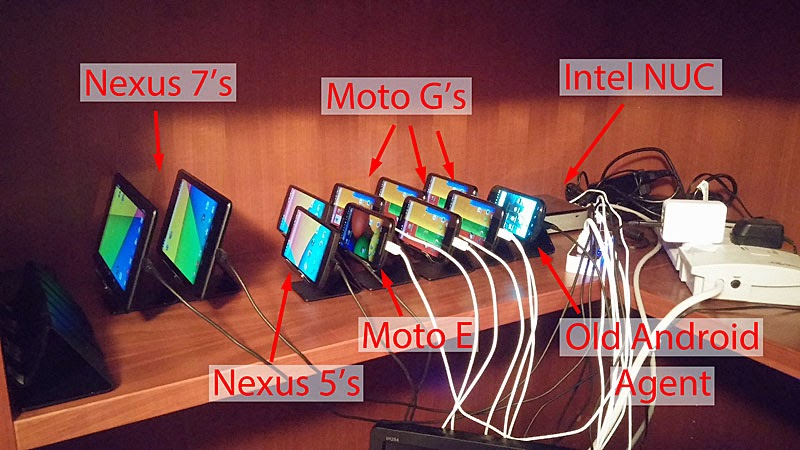
\includegraphics[width=0.5\textwidth]{wpt-android.jpg}
						\caption{Webpagtest Android device farm (Abbildung von \autocite{meenan15})}
						\label{fig:wpt-android}
					\end{center}
				\end{figure}
				\item Webpagetest hat die wohl genauste Erfassung von Netzwerkzeiten und spiegelt damit realitätsgetreu die Ladezeiten einer Seite wieder.

				\item Webpagtest liefer eine enormes Spektrum an Daten und Diagrammen, was ausführliche Analysen zulässt.

				\item Speed Index: Dies ist eine von diesem Tool eigene Maßeinheit zum bestimmen der \texttt{Perceived Performance} einer Seite.

				\begin{quote}
					\textit{"`'The Speed Index metric was added to WebPagetest in April, 2012 and measures how quickly the page contents are visually populated (where lower numbers are better).  It is particularly useful for comparing experiences of pages against each other (before/after optimizing, my site vs competitor, etc) and should be used in combination with the other metrics (load time, start render, etc) to better understand a site's performance."'}\autocite{webpagetestDocs}
				\end{quote}

				\item Man kann Tests direkt miteinander vergleichen. Das ist möglich, indem diese URL eingegeben wird: \url{www.webpagetest.org/video/compare.php?tests=} und nach dem "`="' Zeichen die Test ID eingibt, beispielsweise "`150310\_8E\_GRH"'.
				Mit einem Komma getrennt wird eine 2. oder 3. ID angefügt. Die Tests werden dann in einer Vergleichsansicht dargestellt.

				\item Filmstrip Ansicht: Damit lässt sich visuell erkennen, wann welches Element gerendet wird.

				\item Video erstellung: Aus der Filmstrip Ansicht lässt sich ein Video erstellen. Das ist vor allem interessant, wenn mit der Vergleichsmethode mehrere Tests geladen sind. Der Ladevorgang der Testläufe wird dann in einem Video Parallel abgespielt. Vor allem für Präsentationen oder vorher / nachher Vergleiche ist dies nützlich.

				\item Test History: Durch eine Registrierung auf der Seite wird ein eigenes Testprofil angelegt in dem alle Test-ID's gespeichert werden.

				\item Testen von verschiedenen Standpunkten: Webpagetest ermöglicht es die eigene Seite von ganz verschiedenen Geographischen Standpunkten aus aufzurufen. Dadurch lässt sich ein Eindruck gewinnen, wie schnell die Seite aus dem Ausland aufrufbar ist und wie stark die Abweichung sein kann.

				\item API: Webpagtest hat eine offene API (Schnittstelle) durch die das Tool von außerhalb erreichbar ist. So lässt sich ein Test beispielsweise in Google-Spreadsheets aufrufen und das Ergebnis direkt in eine Tabelle schreiben. Mehr dazu in Punkt: \ref{..} ?. Diese Schnittstelle Limitiert allerdings die Anzahl an Tests pro Tag auf 200. Für mehr muss man sich eine eigene Private Instanz erstellen. 
				%todo ref

				\item Private Instanz: Da webpagetest Open Source ist, gibt es die möglichkeit eine eigene Private Instanz aufzusetzen. Dies kann sowohl per Amazon Cloud oder auf einem eigenen Server geschehen. Damit lassen sich dann soviele Tests ausführen, wie die Leistungs des Servers bietet.

			\end{itemize}
		% subsubsection webpagetest (end)	

		\subsubsection{Pingdom} % (fold)
		\label{ssub:pingdom}
			\url{http://tools.pingdom.com/fpt/} ist eine Alternative zu Webpagetest. Auch damit lässt sich eine URL nach Performanceproblemen analyisieren. Die Ergebnisse sind nicht so genau wie mit Webpagetest und auch ein Testen mit Smartphones fehlt. Bei einer kostenlosen Anmeldung erhält man allerdings ein System zur Überwachung der eigenen Webanwendung. Bei Ausfall oder zu hoher Last kann eine SMS versendet werden um den Admin auf diesen Umstand hinzuweisen. Durch einbetten eines Scripts auf der eigenen Seite lässt sich die Response zeit aufzeichnen (siehe Abbildung \ref{fig:choose_a_good_host}). Dieses tracking nennt man auch "`real user monitoring"' und ist zum Beispiel auch durch Google Analytics in solch einer Form abrufbar.

		
		% subsubsection pingdom (end)

		\subsubsection{Speedcurve} % (fold)
		\label{ssub:speedcurve}
			Ist ein kommerzielles Tool basierend auf Webpagetest. Es liefert einen "`life monitoring"' Service mit dem sich Webanwendungen vergleichen lassen. So kann man zum Beispiel die eigene Webanwendung dauerhaft und über einen längeren Zeitraum mit denen der Konkurenz vergleichen. 

			\begin{figure}[htbp]
				\begin{center}
					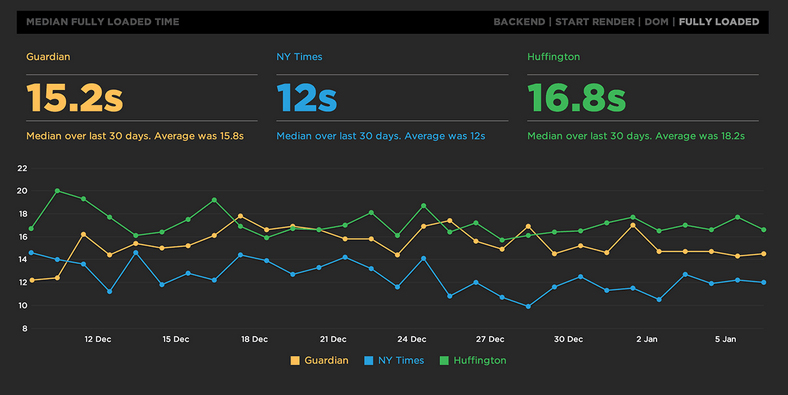
\includegraphics[width=0.7\textwidth]{speedcurve.jpg}
					\caption{Speedcurve Life Monitoring (Abbildung von \url{http://speedcurve.com/})}
					\label{fig:speedcurve}
				\end{center}
			\end{figure}

		% subsubsection speedcurve (end)

		\subsubsection{Google Spreadsheet} % (fold)
		\label{ssub:google_spreadsheet}
			Ist im Grunde wie Microsofts Excel. In Tabellen können Werte eingetragen und Berechnungen ausgeführt werden.
			Der große Vorteil an Google Spreadhseet besteht in der Möglichkeit, dass es einen Skript Editor gibt, mit dem sich kleine Programme schreiben lassen. So sind zum Beispiel API Abfragen möglich, dessen Ergebnis dann direkt in die Tabelle geschrieben werden kann.		
		% subsubsection google_spreadsheet (end)

		\subsubsection{Feed the Bot} % (fold)
		\label{ssub:feed_the_bot}
			\url{http://www.feedthebot.com/pagespeed/} bietet umfassende Artikel zu SEO und web performance. Wenn man sich mit dem Thema web performance beschäftigen möchte, ist dies eine erstklassige Anlaufstelle.
		% subsubsection feed_the_bot (end)


		\subsubsection{What Does My Site Cost?} % (fold)
		\label{ssub:what_does_my_site_cost}
			"`Was kostet es eigentlich meinene Seitenbesucher, wenn sein Datenvolumen für diesen Monat aufgebraucht ist und er pro verbrauchtes MB zur Kasse gebeten wird?"' Diese Frage versucht diese Webanwendung zu klären und visuell darzustellen.\\
			\url{http://whatdoesmysitecost.com/} benutzt die webpagetest Schnittstelle um eine eingegebene URL zu Analyisieren und berechnet aus den billigsten Anbieteren pro Land einen Preis für den Aufruf der Seite mittels Smartphone:

			\begin{quote}
				\textit{"`Prices were collected from the operator with the largest marketshare in the country and the for the least expensive plan with a (minimum) data allowance of 500 MB over (a minimum of) 30 days. Prices include taxes. Because these numbers are based on the least expensive plan, they are \textbf{best case} scenarios."'}\autocite{siteCosts}
			\end{quote}

		\begin{figure}[htbp]
			\begin{center}
				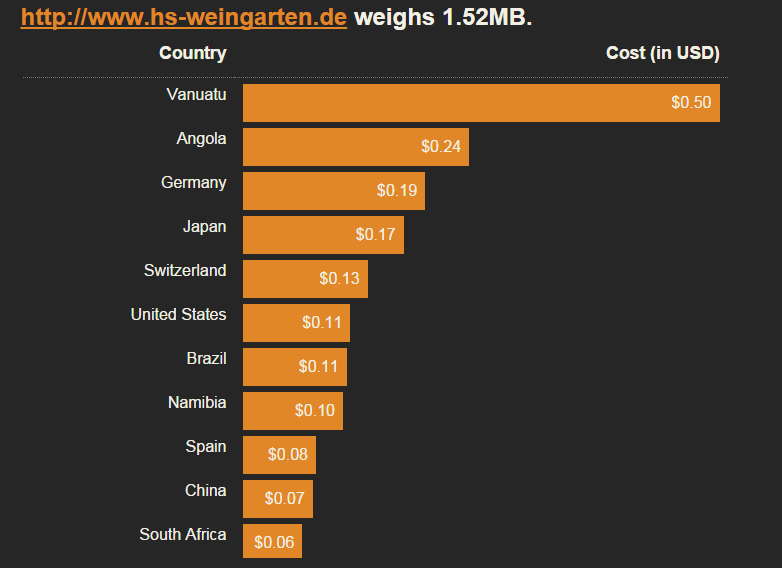
\includegraphics[width=0.7\textwidth]{what_does_my_site_cost.jpg}
				\caption{Find out how much it costs for someone to use your site on mobile networks around the world.\autocite{siteCosts}}
				\label{fig:what_does_my_site_cost}
			\end{center}
		\end{figure}

		In Deutschland kostet also der Seitenaufruf von hs-weingarten.de rund 20 Cent. Dieses Tool stellt auf sehr schöne Art und Weise dar, dass schlechte web performance nicht nur den Anwender verägert, sondern zusätzlich zum Ärger auch noch bares Geld kosten kann.
		% subsubsection what_does_my_site_cost (end)

		\subsubsection{Critical Path CSS Generator} % (fold)
		\label{ssub:critical_path_css_generator}
			Im Kapitel "`Brechen der 1000 ms Barriere"'\ref{sec:die_1000_ms_barriere} wurde gesagt, man solle das CSS des above the folds direkt in das HTML als \texttt{inline CSS} schreiben. \url{http://jonassebastianohlsson.com/criticalpathcssgenerator/} erstellt aus einer gegebener URL und dem dazugehörigen CSS genau den CSS-Code, der für den above the fold Bereich nötig ist. Das Ergebnis lässt sich dann bequem in das eigene HTML einfügen.\\

			Dieser Generator funktioniert allerdings nur dann gut, wenn sowohl die Smartphone, als auch Desktop Darstellung identisches CSS haben. Bootstrap zum Beispiel manipuliert die Navigation auf der Smartphone Ansicht per Javascript und fügt dabei Elemente ein. Diese Elemente kennt dieser Generator natürlich nicht und kann sie folglich auch nicht beachten. Eine alternative Methode wird in Kapitel ... \ref{..} ? vorgestellt.

		% subsubsection critical_path_css_generator (end)

		\subsubsection{Http Archive} % (fold)
		\label{ssub:http_archive_bigqueri_es}
			\url{http://httparchive.org/} ist ein Archiv der populärsten Seiten des Internets und bietet eine Vielzahl an statistischen Auswertungen, Trends und Daten.
			\begin{quote}
				\textit{"`[HTTP Archive] is a permanent repository of web performance information such as size of pages, failed requests, and technologies utilized. This performance information allows us to see trends in how the Web is built and provides a common data set from which to conduct web performance research."' \autocite{httpArchive}}
			\end{quote}
			
		% subsubsection http_archive_bigqueri_es (end)

		\subsubsection{Perf Tooling Today} % (fold)
		\label{ssub:perf_tooling_today}
			\url{http://perf-tooling.today/} ist wohl die Umfassendste Sammlung an web performance Tools und Material im Internet. Es hat eine Liste von 105 Tools, 51 Artikel, 27 Videos und 14 Slidedecks (Stand: 12.03.15).
		
		% subsubsection perf_tooling_today (end)

		\subsubsection{Twitter} % (fold)
		\label{ssub:twitter}
			Twitter bietet die Möglichkeit am Puls der Zeit zu sein und unter dem Hashtag \#webperf und \#perfmatters erhält man neuste Erkentnisse, Tools oder Links, die sonst unentdeckt bleiben.
		
		% subsubsection twitter (end)
	\pagebreak
	% subsection tools (end)


	\subsection{Ausgangspunkt}
	\label{sub:ausgangspunkt}
		Im folgenden Abschnitt soll der Prozess beschrieben werden, um von einer langsamen Webanwendung zu einer schnellen zu gelangen. Von Beginn an war es wichtig, den Verbesserungsablauf zu Dokumentieren und in konkrete Daten zu fassen. Wie bereits unter Punkt \ref{ssub:google_spreadsheet} beschrieben, bietet Google Spreadsheets die möglichkeit Skripte zu schreiben und die Ergebnisse direkt in eine Tabelle auszugeben. Diesen Umstand hat sich \texttt{Andy Davies} zu nutzen gemacht und ein Programm\footnote{WebPageTest Bulk Tester via GitHub: \url{https://github.com/andydavies/WPT-Bulk-Tester}} geschrieben (MIT License), dass es ermöglicht Webpagtestest innerhalb einer Google Tabelle\footnote{Das Google Dokument ist hier zu finden: \url{http://tinyurl.com/nv4pge5}} aufzurufen. Damit wurde während der Entwicklungsphase täglich tests aufgezeichnet.\footnote{Die gesamten Daten sind hier zu finden: \url{http://tinyurl.com/l5usz79}} Die Auswertung dieser Daten erfolgt in Punkt \ref{..} ?\\
		%todo ref

		Da nur in Dulles VA eine Testinstanz mit richtigen Smartphones zur Verfügung steht, wurde mittels der \texttt{Microsoft Azure Cloud} die selbe Seite auch in den USA gehostet, um die Latenz zwischen USA und Europa zu eliminieren. Dadurch lässt sich exakter bestimmen, wie schnell ein Smartphone mit 3G Netz die Seite aufrufen kann. Leider steht keine Testinstanz mit 4G Netz zur Verfügung.\\

		Als Ausgangspunkt dient die Seite \url{http://andreaslorer.de/old/}. Zu beginn des Optimierungsprozesses gab es folgenden Ausgangspunkt (Daten via Developer Tool \& webpagetest):\\

		Desktop: \footnote{Webpagtest: \url{http://www.webpagetest.org/result/150312_Z1_18QD/}}
		\begin{itemize}
			\item 42 requests: 30 Images, 5 JS, 3 CSS, 4 other
			\item 1000 kb Seitengröße
			\item Speed Index: \textbf{3584}
			\item Start Render: \textbf{1399}  ms
			\item Load Time: 1926 ms
			\item TTFB: 690 ms
		\end{itemize}

		Mobile: \footnote{Webpagtest: \url{http://www.webpagetest.org/result/150308_A1_2W4/}}
		\begin{itemize}
			\item 17 requests: 4 Images, 5 JS, 3 CSS, 4 other
			\item 363 kb Seitengröße
			\item Speed Index: \textbf{10642}
			\item Start Render \textbf{6968} ms
			\item Load Time: 5587 ms
			\item TTFB: 1292 ms
		\end{itemize}

		Diese Werte sind nicht gut und für dieses Projekt wurden eine Start Render Zeit von weniger als einer Sekunde und ein Speed Index von unter 1000, für sowohl Mobile- als auch Desktopgeräte, angestrebt.\\

		Der erste Schritt war es, die Seitengröße zu verringern. Aus diesem Grund wurde das Framework gewechselt und die Seite neu Aufgebaut. Bootstrap ist zwar ein sehr populäres Framework, hat aber gerade für kleine Seiten sehr viele Komponenten, die keine Verwendung finden (oft auch als Overhead bezeichnet). Bootstrap lässt sich zwar per "`Customize"' Funktion so zusammenstellen, dass nur die Komponenten zur Verfügung gestellt werden, die für das eigene Projekt von Nöten sind, es ist aber dennoch ein Framework mit relativ großem Volumen (~30 bis 90 kb). Die Alternativen zu Bootstrap sind vielzählig. Die Entscheidung für dieses Projekt fiel auf \url{http://purecss.io/}. Dieses Framework von Yahoo ist Komprimiert gerade einmal \textbf{4 kb} groß, vollkommen responsive und kommt mit den wichtigsten Komponenten wie einer Navigations Bar, Buttons, Tabellen, Menüs und Form Elementen. Je nach gewählten Komponenten, benötigt es kein Javascript und kein JQuery. Dadurch lassen sich weitere Kilobytes als auch Requests einsparen.\\
		Da Bootstrap seine eigene Icon-Font liefert, musste hier eine Alternative gefunden werden. "`Font Awesome"'\footnote{Font-Awesome: \url{http://fortawesome.github.io/Font-Awesome/}} bietet dabei eine der umfangreichsten Icon Sammlungen im Web an und ist unter der \texttt{Open Font License} komplett frei benutzbar (auch kommerziell). Font Awesome ist mit seinen 519 Icons allerdings nicht gerade ein Leichtgewicht und kann bis zu 100 kb groß sein. Da auf der Seite \url{http://andreaslorer.de} weniger als 20 Icons zum Einsatz kommen ist der Überschuss folglich enorm. Deshalb gibt es eine Webanwendung namens \url{http://fontello.com}. Damit lassen sich aus einer Vielzahl an Icons genau die wählen, die für die eigene Seite benötigt werden. Auch das Wählen aus verschiedenen Icon-Sammlungen ist möglich. Heruntergeladen wird anschließend eine ZIP-Datei. Das Resultat: Die neue Version der Seite benötigt nur noch 5.6 kb für die Icons. Verglichen mit: Bootstrap 43 kb, Font-Awesome 97 kb.\\

		Als nächstes wird die Webanwendung mittels \texttt{Pagespeed Insight}\ref{ssub:google_pagespeed_insight} Analyisert. Das Ergebnis liefert Anhaltspunkte, was für schnellere Ladezeit alles umgesetzt werden sollte. Im folgenden soll erläutert werden, was es alles an Verbesserungen gibt und wie eine mögliche Umsetzung in der Praxis aussieht.

		% zusammenfügen mit best practices?

		\subsubsection{Render Blocking Javascript} % (fold)
		\label{ssub:render_blocking_javascript}
			Bereits unter Punkt \ref{ssub:rendering_pfad} ist das Blockierende Verhalten von Javascript und CSS angesprochen worden. Grundvoraussetzung für diesen Punkt ist, dass das Javascript der Webanwendung in ihre, für das Rendern kritische und für das Rendern unkritische Teile zerlegt wurde. 

			Der Browser stellt bereits von Haus aus zwei Attribute bereit, mit denen sich Skripte asynchron herunterladen lassen. Diese Attribute heißen "`async"' und "`defer"' und werden von jedem Browsertyp unterstützt.\autocite{canIuse} Sie erlauben es, dass der Browser nicht auf das Herunterladen der Dateien warten muss, sondern mit dem Parsen des Dokuments fortfahren darf. Async wird direkt nach dem herunterladen ausgeführt und dafür muss das Parsen pausiert werden. Defer hingegen unterscheidet sich von async in zwei Punkten: 1. Das Skripte wird nach Ende des Parsens ausgeführt. 2. Mit defer verzögert geladene Skripte werden in genau der Reihenfolge ausgeführt, wie die Reihenfolge der Skripte im HTML Dokuments vorliegen.
			
			\begin{figure}[htbp]
				\begin{center}
					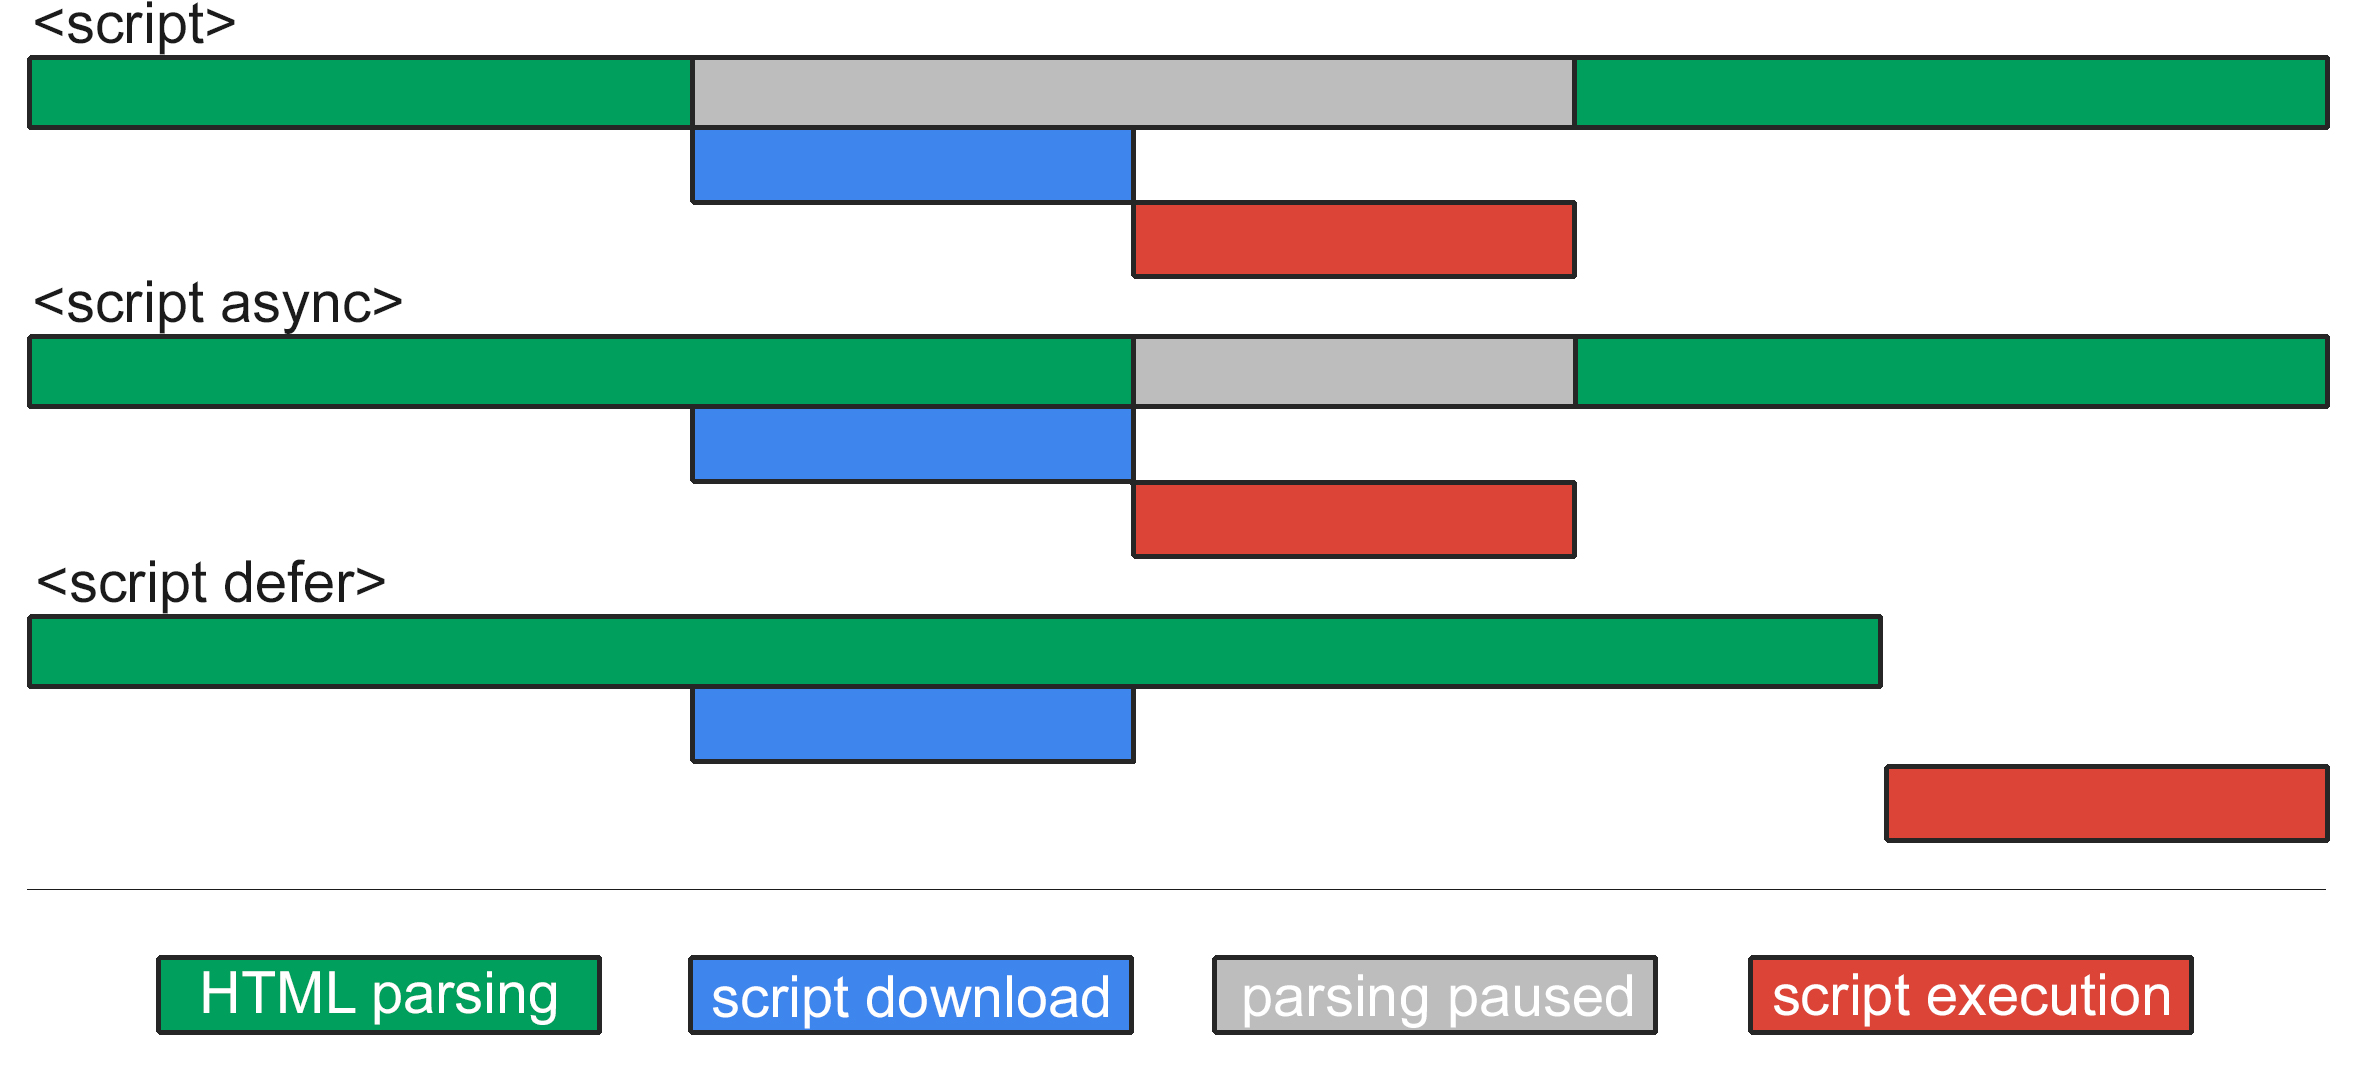
\includegraphics[width=\textwidth]{defer_scripts.jpg}
					\caption{Script-Tags mit verschiedenen Attributen (Abbildung nach \autocite{growing})}
					\label{fig:defer_scripts}
				\end{center}
			\end{figure}

			Diese Methode erlaubt es, Skripte parallel herunterzuladen, ohne dass der Renderprozess warten muss. Was damit nicht erreicht werden kann ist, dass der Download so lange verzögert wird, bis die für die Seiten primär wichtigen Ressourcen zuerst heruntergeladen wurden.\\

			Mit Hilfe des Javascripts in Listing \ref{lst:deferJs}, kann die Datei "`defer.js"' komplett mit dem Laden verzögert werden, bis der Ladeprozess der Seite abgeschlossen ist.\\
	
			\begin{lstlisting}[captionpos=b, caption=Javascript nach \autocite{deferJS}, label=lst:deferJs]
			// the function to asynchronous load js
			function loadJS( src, cb ){
				"use strict";
				var ref = window.document.getElementsByTagName( "script" )[ 0 ];
				var script = window.document.createElement( "script" );
				script.src = src;
				script.async = true;
				ref.parentNode.insertBefore( script, ref );
				if (cb && typeof(cb) === "function") {
					script.onload = cb;
				}
				return script;
			}

			// the function call to load your script
			loadJS( "path/to/script.js" );
			\end{lstlisting}

			Dieses Skript hat einen Nachteil: Es kann nicht mehrere Skripte laden, die voneinander Abhängen und deren Reihenfolge wichtig ist, um die Funktionalität zu gewährleisten. 

			\begin{quote}
				\textit{"`loadJS does nothing to manage execution order of requested scripts, so we do not advise using it to load multiple javascript files that depend on one another. It simply fetches a script and executes it as soon as possible. You can certainly use loadJS to load multiple scripts as long as those scripts are designed to execute independently of any other scripts being loaded by loadJS."'\autocite{deferJS}}
			\end{quote}

			So gibt es Skripte (Skript A) die von anderen Frameworks wie zum Beispiel JQuery (Skript B) abhängen. Das bedeutet, wenn Skript A schneller heruntergeladen und ausgeführt wird als Skript B, A bereits Funktionen von B aufruft, die noch nicht zur Verfügung stehen. Daraus resultiert ein Fehlschlagen des Skripts und somit können teile der Webanwendung nicht mehr wie beabsichtigt Funktionieren.\\

			Darum gibt es Skripte die genau diese Funktionalität bereitstellen können. Skript A und B werden gleichzeitig heruntergeladen, A wird aber erst genau dann Ausgeführt, wenn B zur Verfügung steht.\\

			\url{http://headjs.com/} kann das erreichen. Durch das Herunterladen und Einfügen in das HTML Dokument, kann per Funktionsaufruf die Abhängigkeit festgelegt werden:

			\begin{lstlisting}[captionpos=b, caption=Headjs dependency loading (Listing nach http://headjs.com/), label=lst:headjs]
				// Load up some script A and then script B
				head.load("jQuery.js", function() {
				    // Call a function when done
				    console.log("Done loading jQuery");
				    head.load('defer.js')
				});
			\end{lstlisting}

			Headjs hat den Nachteil, dass es auch noch andere Funktionalitäten außer dem Laden von Javascript ermöglicht. Dies wird aber nicht benötigt und deshalb ist Headjs mit 2.1 kb doch zu groß, um es \texttt{Inline} in das HTML Dokument zu schreiben. Eine bessere Alternative ist \texttt{jQl}. \footnote{jQl an asynchronous jQuery Loader: \url{http://www.yterium.net/jQl-an-asynchronous-jQuery-Loader}}
			Die Verwendung ist sehr Simpel:

			\begin{lstlisting}[captionpos=b, caption=jQl asynchronous jQuery-Loader, label=lst:jQl]
				<script type="text/javascript">
					// first include jQl inline (missing here) then call these functions
				  jQl.loadjQ('jquery.js');
				  jQl.loadjQdep('defer.js');
				</script>
			\end{lstlisting}

			Dieses Skript sagt im Grunde: Lade beide Dateien gleichzeitig herunter, beachte aber die Abhängigkeit (loadjQdep steht für: load dependency) von defer.js gegenüber JQuery. Ist defer.js früher heruntergeladen als JQuery, so wird gewartet und anschließend werden die Skripte in der richtigen Reihenfolge ausgeführt.\\

			Für die Webseite \url{http://andreaslorer.de} wurde sowohl defer, als auch das Skript \texttt{jQl} verwendet. "`<script defer src='critical.js'></script>"' wird dabei in den "`<head>"' bereich des HTML Dokments platziert, damit es möglichst früh erkannt wird und der Download bereits beginnen kann und das Skript aus Listing \ref{lst:jQl} befindet sich vor dem "`</body>"'-Tag.

			\pagebreak

		% subsubsection render_blocking_javascript (end)

		\subsubsection{Render Blocking CSS} % (fold)
		\label{ssub:render_blocking_css}
			Wie Javascript blockiert auch CSS das Rendern der Seite. In Listing \ref{deferCSS} ist ein Skript der Filament Group uzu sehen. Dieses Skript ermöglicht es CSS Verzögert zu laden. 

			\begin{lstlisting}[captionpos=b, caption=load a CSS file asynchronously, label=lst:deferCSS, breaklines=false]
			<script>
				// minified script after: 
				// https://github.com/filamentgroup/loadCSS/blob/master/loadCSS.js
				// [c]2014 @scottjehl, Filament Group, Inc.
				// Licensed MIT
	 			function loadCSS(e,a,g,h){function f(){for(var a,c=0;c<d.length;c++)d[c].href&&
	 				-1<d[c].href.indexOf(e)&&(a=!0);a?b.media=g||"all":setTimeout(f)}
	 				var b=window.document.createElement("link");a=a||
	 				window.document.getElementsByTagName("script")[0];
	 				var d=window.document.styleSheets;b.rel="stylesheet";b.href=e;b.media="only x";
	 				b.onload=h||function(){};a.parentNode.insertBefore(b,a);f();return b
	 			};

	  		loadCSS( "path/to/css" );
			</script>

			<!-- fallback if javascript is disabled in browser -->
			<noscript><link href="path/to/css"></noscript>
			\end{lstlisting}

			Mehr als dieses Skript ist nicht notwendig.
				
		% subsubsection render_blocking_css (end)

		\subsubsection{Inline von CSS} % (fold)
		\label{ssub:inline_von_css}
			Kleinere Mengen an CSS lassen sich direkt \texttt{Inline} in das HTML Dokument einfügen. Dadurch sind diese gleich mit dem ersten Request bereits im Dokument enthalten und müssen nicht erst angefordert und heruntergeladen werden.
		% subsubsection inline_von_css (end)

		\subsubsection{Ressourcen reduzieren} % (fold)
		\label{ssub:ressourcen_reduzieren}
			Das schnellste Byte ist das, dass nicht gesendet wird und der schnellste Request ist der, der nicht gestellt wird. Deshalb gibt es drei Maßnahmen die für eine Webanwendung umgesetzt werden sollte:

			\begin{itemize}
				\item "`Minify"': Kommentare, Leerzeichen oder Zeilenumbrüche sind für die Funktionalität nicht notwendig. Bei der Verkleinerung des HTML- CSS oder Javascript Codes werden diese entfern und dadurch die Dateigröße verkleinert. Wie unter Punkt \ref{ssub:google_pagespeed_insight} angesprochen, gibt es Pagespeed Insight auch als Chrome-Erweiterung. Damit ist es möglich, eine reduzierte Version des HTML Dokuments zu erzeugen. Für Javascript ist der Closure Compiler (\ref{ssub:closure_compiler}) das richtige Werkzeug. CSS lässt sich per \url{http://cssminifier.com/} verkleinern.
				\item "`Uglify"': Dabei werden Variablennamen, auf nur wenige Zeichen reduziert. Aber auch Code wird teilweise umgeschrieben, wenn für einen verwendeten Ausdruck beispielsweise eine kürzere Schreibweise existiert.

				\begin{lstlisting}[captionpos=b, caption=Beispiel: Uglify eines Ausdrucks, label=lst:uglify]
				// input:
				if(foo){
					bar();
				}
				else{
					boo();
				}

				// output:
				foo?bar():boo();
				\end{lstlisting}

				Input und Output sind identisch in ihrem Ausdruck, die Zeichenanzahl wurde aber von 27 auf 16 verringert.

				\item "`Concatenate"': Damit ist das Zusammenfügen von einzelnen Dateien zu einer Einzigen gemeint. Dadurch lassen sich zusätzliche Requests einsparen. Dies hat den Vorteil, dass sowohl der TCP Slow start nur einmal eintritt als auch nur eine TCP Verbindung aufgebaut werden muss. Zusätzlich werden weniger TCP Verbindungen belegt, denn dafür gibt es, wie bereits erwähnt wurde (Punkt \ref{sub:http_1_1}), ein Limit.
			\end{itemize}
		% subsubsection ressourcen_reduzieren (end)

		\subsubsection{CSS-Bereitstellung optimieren} % (fold)
		\label{ssub:css_bereitstellung_optimieren}
			Wenn externe Ressourcen klein sind, können diese direkt in das HTML Dokument \texttt{Inline} platziert werden. Dabei sollte darauf geachtet werden, dass das HTML Dokument Komprimiert nicht die 14 kb Marke überschreitet. Dadurch kann es im ersten round trip geliefern werden. CSS Dateien die groß sind sollten per \texttt{Link-Tag} eingebunden werden und mittels Skript Verzögert geladen werden. Das CSS für den above the fold Bereich sollte \texttt{Inline} im "`<head>"' Bereich der Seite stehen. 
		% subsubsection css_bereitstellung_optimieren (end)

		\subsubsection{Antwortzeit des Servers reduzieren} % (fold)
		\label{ssub:antwortzeit_des_servers_reduzieren}
			Die Zeit zur Antwort des Servers lässt sich zum Beispiel mit Webpagtest herausfinden. Ein Server sollte auf eine Response Zeit von unter 200 ms kommen. \textit{"`Es gibt Dutzende potenzielle Faktoren, die die Antwortzeit Ihres Servers beeinträchtigen können: eine langsame Anwendungslogik, langsame Datenbankabfragen, langsames Routing, Frameworks, Bibliotheken, CPU-Ressourcenmangel oder Speicherplatzmangel. Berücksichtigen Sie zur Verkürzung der Antwortzeit Ihres Servers alle diese Faktoren."'} \autocite{google15}. Bereits unter Punkt: \ref{sub:zusammengefasst} wurde es nahegelegt ein gutes Hosting zu wählen. Besser Sie wechseln ihr Hosting als ihre Kunden den Service.
		% subsubsection antwortzeit_des_servers_reduzieren (end)

		\subsubsection{Browser-Caching nutzen} % (fold)
		\label{ssub:browser_caching_nutzen}
			Fehlendes Browser-Caching (das lokale Speichern von Daten) wird von Pagspeed Insight bemängelt, wenn der Server bei seiner Antwort keinen expliziten \texttt{Caching-Header} versendet.
			Durch das Speichern von statischen Ressourcen wie Javascript, Stylesheets und Bildern kann Zeit eingespart werden, wenn der Besucher die Webanwendung ein weiteres mal aufruft. Generell sollten alle statischen Ressourchen außer das HTML Dokument selbst, gechached werden.\\

			Um auf dem Server (Apache) das Caching von statischen Ressourcen zu ermöglichen, ist ein Eintrag in die \texttt{htaccess} Datei des Servers nötig. Folgender Eintrag sollte dort platziert werden:

		  \begin{lstlisting}[captionpos=b, caption=Aktivieren von Browser Caching in Apache (Listing nach: \autocite{sextonCaching}), label=lst:caching, language=bash]
		  	## EXPIRES CACHING ##
		  	<IfModule mod_expires.c>
		  	ExpiresActive On
		  	ExpiresByType image/jpg "access 1 year"
		  	ExpiresByType image/jpeg "access 1 year"
		  	ExpiresByType image/gif "access 1 year"
		  	ExpiresByType image/png "access 1 year"
		  	ExpiresByType text/css "access 1 year"
		  	ExpiresByType text/woff "access 1 year"
		  	ExpiresByType application/pdf "access 1 year"
		  	ExpiresByType text/x-javascript "access 1 year"
		  	ExpiresByType application/x-shockwave-flash "access 1 year"
		  	ExpiresByType image/x-icon "access 1 year"
		  	ExpiresDefault "access 1 month"
		  	</IfModule>
		  	\#\# EXPIRES CACHING \#\#
		  \end{lstlisting}

		  Listing \ref{lst:caching} hat 2 Aufgaben. Erstens: Es setzt die Ablaufzeit für alle statischen Ressourcen auf 1 Jahr und erfüllt damit den von Google empfohlenen Wert. Längere Speicherzeiten sind dagegen nicht Empfohlen, da dies gegen die RFC-Richtlinien verstoßen würde \autocite{google14Caching}. Zweitens: Es wird mit dem HTTP Request ein Header mit gesendet. Dieser ermöglicht es dem Browser seine lokal gespeicherten Ressourcen zu managen. Er besteht aus folgenden Teilen und es ist jeweils nur \textbf{eine} der Optionen nötig.

		  \begin{itemize}
		  	\item Last-Modified: date
		  	\item ETag: ID
		  \end{itemize}

		  Diese beiden Header ermöglichen es dem Browser zu überprüfen, ob sich die gecachten Ressourcen geändert haben oder noch identisch sind. Last-Modified ist dabei das Datum der letzten Änderung und der ETag-Header ist ein automatisch generierter Wert, der die Datei eindeutig Identifiziert.\\
		  Beim erneuten Laden einer Seite werden diese Header zurück an den Server gesendet und verglichen. Wenn die Datei auf dem Server geändert wurde stimmen die Werte nicht überein und der Server schickt eine entsprechende Antwort zurück.

		  \begin{itemize}
		  	\item Cache-Control: max-age=value
		  	\item Expires: date
		  \end{itemize}

		  Mit diesen Headern ist es möglich Serveranfragen komplett zu vermeiden. "`Sämtliche vom Browser ausgegebenen HTTP-Anfragen werden zuerst an den Browsercache weitergeleitet, um zu überprüfen, ob eine gültige Antwort im Cachespeicher vorliegt, die der Anfrage entspricht. Liegt eine Übereinstimmung vor, wird die Antwort aus dem Cache ausgelesen, wodurch sowohl die Netzwerklatenz als auch die durch die Übertragung anfallenden Datenkosten umgangen werden."'\autocite{grigorikCaching} Das bedeutet, dass die Latenz bei Smartphones für gecachte Dateien komplett negiert werden kann. Gültige Ressourcen werden erst gar nicht angefragt, sondern gleich aus dem Cache geladen. Ungültige oder abgelaufene Ressourcen werden dagegen vom Server geholt. Ohne diesen Header, muss der Browser für jede in seinem Cache befindliche Ressource, den Server anfragen. Dafür sind jedes mal ein round trip nötig.\\

		  \begin{figure}[htbp]
		  	\begin{center}
		  		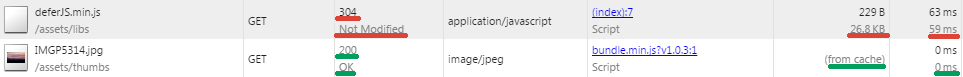
\includegraphics[width=\textwidth]{caching_enabled.jpg}
		  		\caption{Gecachte Ressourcen müssen nicht mehr abgefragt werden}
		  		\label{fig:caching_enabled}
		  	\end{center}
		  \end{figure}
		  
		  Das rot unterstrichene zeigt, dass 59 ms im Netzwerk verbraucht wurde (Kabel Verbindung). Der Server antwortete mit: "`Not-Modified"'. Grün zeigt, dass keinerlei Kommunikation mit dem Server nötig ist sondern die Datei, in diesem Fall ein Bild, direkt aus dem Cache geholt wird.\\
		  Fazit: Ohne Cache-Control lässt sich durch die Browser eigene Caching Funktionalität das erneute Herunterladen der Datei vermeiden. Mit Cache-Control kann sowohl das Herunterladen als auch der gesamte Verbindungsaufbau zum Server vermieden werden.\\
		 
		  Was aber wenn sich zum Beispiel eine CSS-Datei geändert hat? Dann würden nun Besucher mit leerem Cache eine andere Darstellung erhalten, wie Besucher mit der gecachten Version. Dafür gibt es mehrere Lösungsansätze.

		  \begin{enumerate}
		  	\item Die HTML Datei sollte nicht gecached werden da sonst Änderungen nicht mehr den Anwender können.
		  	\item Eine für die Datei angemessene max-age: Dateien die sich oft ändern dürfen auch entsprechend niedrige max-age Werte haben. Dadurch wird die Datei Zeitnah für alle Anwender neu Angefordert.
		  	\item Ressourcen können mit einer ID versehen werden: \texttt{styles.css} wird in \texttt{styles.v1.0.1.css} umbenannt.
		  	\item Alternativ zur ID ist auch in \texttt{Fingerprint} möglich. Dabei wird eine ID aus der Datei generiert. Ändert sich die Datei so ändert sich auch der Fingerprint. Dieser Fingerprint wird auch wiederrum dem Dateiname angefügt. Das kann so aussehen: \texttt{styles.82s0dfsa.css}.\footnote{Dieses Verfahren lässt sich auch automatisieren, ich verweise auf folgenden Artikel: \url{https://adactio.com/journal/8504}}
		  \end{enumerate}

		  Browser-Caching ist eine mächtige Funktionalität die sich jeder zu nutzen machen sollte. Sie ist zudem ganz einfach mit nur einem Eintrag in die \texttt{htaccess}-Datei realisierbar. Allerdings hat eine Studie von Yahoo ergeben, dass 40-60\% der Besucher beim Seitenaufruf einen leeren Cache haben und rund 20\% aller aufgerufenen Seiten wurden mit einem leeren Cache aufgerufen.
			\begin{quote}
				\textit{"`[...] I don't know about you, but these results came to us as a big surprise. It says that even if your assets are optimized for maximum caching, there are a significant number of users that will always have an empty cache."'\autocite{yahoo07}}
			\end{quote}

			Folglich macht es Sinn, die Geschwindigkeit der Seite für die sogenannten "`first users"' zu optimieren und nicht von einem gecachten Zustand der Seite auszugehen.\\
			\texttt{Feed-The-Bot} stellt ein Tool\footnote{Tool: \url{http://www.feedthebot.com/tools/if-modified/}} zu Verfügung, mit dessen Hilfe sich überprüfen lässt, ob die eigene Webseite "`Browser-Caching"' richtig einsetzt. Abbildung Nummer \ref{fig:expires_header} zeigt Links eine Seite mit aktiviertem Browser-Caching und Rechts eine Seite ohne.
		  \begin{figure}[htbp]
		  	\begin{center}
		  		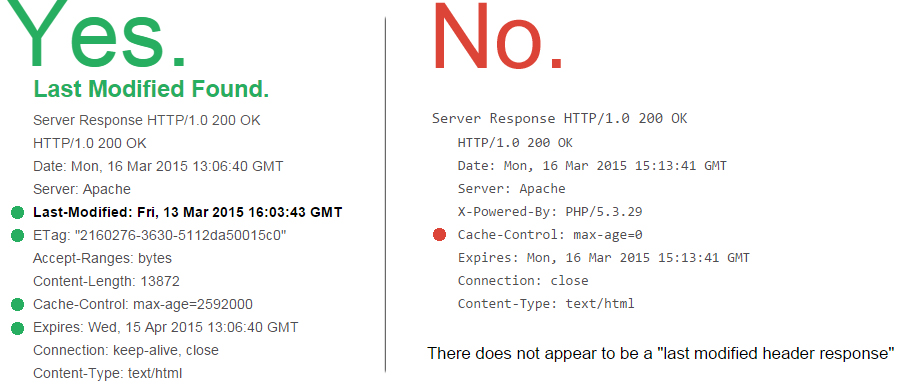
\includegraphics[width=\textwidth]{expires_header.jpg}
		  		\caption{Beispiel: Eine Webseite mit und ohne "`Cache Control"'. (Eigene Abbildung nach feedthebot.com)}
		  		\label{fig:expires_header}
		  	\end{center}
		  \end{figure}
		% subsubsection browser_caching_nutzen (end)
		\pagebreak

		\subsubsection{Komprimierung aktivieren} % (fold)
		\label{ssub:komprimierung_aktivieren}
			Nachdem durch das in Punkt \ref{ssub:ressourcen_reduzieren} beschriebene Verfahren die Ressourcen soweit wie möglich verkleinert wurden, können diese vor dem Versenden komprimiert werden. Dies nennt man auch Datenkomprimierung und stellt ein ganz eigenes Forschungsgebiet dar. Deshalb soll nur der Grundgedanke erklärt werden.

			Gegeben sei folgende Textnachricht:
			\begin{lstlisting}[captionpos=b, caption=, label=lst:]
# Lorem ipsum dolor sit amet, consectetur adipisicing elit. Debitis temporibus incidunt id.
# Cumque molestiae est praesentium magnam, fugit ipsa.
format: text/plain
date: 21.03.15
AAAZZBBBBEEEMMM EEETTTAAAA
			\end{lstlisting}

			Diese Nachricht ist 200 Zeichen lang und kann durch einfache Regeln verkürzt werden. Zuerst werden die Kommentare, die mit \# gekennzeichnet sind entfernt, denn sie sind für die Bedeutung der Nachricht nicht relevant. Das Datum könnte in eine ID konvertiert werden: 210315. Die Nutzdaten der Nachricht wird nach Wiederholungen durchsucht. Daraus ergibt sich dann: 3A2Z4B3E3M 3E3T4A \autocite{grigorikGzip}. Die Neue Nachricht:

			\begin{lstlisting}[captionpos=b, caption=, label=lst:]
format: text/plain
date: 210315
3A2Z4B3E3M 3E3T4A
			\end{lstlisting}

			Die Zeichenanzahl wurde von 200 Zeichen auf 47 Zeichen reduziert. Das ist eine Reduktion von 76,5\%!			

			Das gängigste Komprimierungsprogramm im Web ist GZIP und wird von allen modernen Browsern unterstützt. Es arbeitet nach dem "`Deflate"'-Algorithmus und Komprimiert Daten verlustlos.\footnote{Eine ausführlichere Beschreibung über den GZIP Algorithmus und der textbasierter Dokumentkomprimierung ist hier zu finden: \url{http://www.infinitepartitions.com/art001.html}. Für ein tiefere Verständnis bietet sich dieses Video von Google an: \url{http://tinyurl.com/mfxt5zt}} Je länger eine Textdatei ist, umso drastischer kann sich die Komprimierung auswirken. GZIP ist meistens Standardmäßig aktiviert. Falls nicht kann GZIP mittels \texttt{htaccess} Eintrag von Listing \ref{lst:gzip} in Apache aktiviert werden.\footnote{Für andere Server wie zum Beispiel Nginx oder Node.js gibt es auf GitHub fertige Konfigurationen \url{https://github.com/h5bp/server-configs}} Einträge in die \texttt{htaccess}-Datei sollten nur dann eingesetzt werden, wenn man zum Beispiel ein Shared Hosting verwendet und dadurch keinen direkten Zugang zur Serverkonfiguration hat. Grund dafür ist, dass die Konfiguration von Apache mittels htaccess den Server verlangsamt.\autocite{apache}

			\begin{lstlisting}[captionpos=b, caption=gzip, label=lst:gzip, language=bash]
				## gzip Compression if availiable
				<ifModule mod_gzip.c>
				mod_gzip_on Yes
				mod_gzip_dechunk Yes
				mod_gzip_item_include file \.(html?|txt|css|js|php|pl)$
				mod_gzip_item_include handler ^cgi-script$
				mod_gzip_item_include mime ^text/.*
				mod_gzip_item_include mime ^application/x-javascript.*
				mod_gzip_item_exclude mime ^image/.*
				mod_gzip_item_exclude rspheader ^Content-Encoding:.*gzip.*
				</ifModule>
			\end{lstlisting}

			Mittels \url{http://www.feedthebot.com/tools/gzip/} lässt sich überprüfen, ob der eigene Server GZIP erlaubt.

			\begin{figure}[htbp]
				\begin{center}
					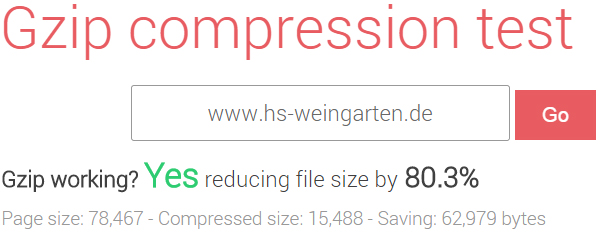
\includegraphics[width=0.5\textwidth]{gzip_compression.jpg}
					\caption{Testen von GZIP anhand von andreaslorer.de (Eigene Abbildung nach: feedTheBot.com)}
					\label{fig:gzip_compression}
				\end{center}
			\end{figure}

			Diesem Tool sollte aber nicht einfach nur blind vertraut werden. Es gibt Ressourcen die müssen explizit als Komprimierbar gekennzeichnet werden. So sollte mittels dem "`Chrome Developer Tool"' (oder vergleichbare Tools wie z.B. Firebug in Firefox) nachgesehen werden, ob alle Ressourcen auch tatsächlich mittels GZIP komprimiert werden. Abbildung \ref{fig:gzip_json} zeigt, dass die Datei: "`Gallery.php"' trotz aktiviertem GZIP keine Komprimierung verwendete.

			\begin{figure}[htbp]
				\begin{center}
					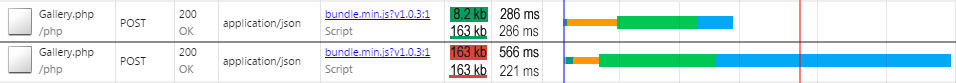
\includegraphics[width=\textwidth]{gzip_json.jpg}
					\caption{Die Serverantwort im JSON-Format ohne und mit GZIP}
					\label{fig:gzip_json}
				\end{center}
			\end{figure}

			Der unterstrichene Wert ist dabei die Datengröße vor GZIP und der farblich hinterlegte Wert nach GZIP. Wie zu sehen ist konnte die zu übertragende Datengröße um fast das 20-Fache verringert werden! Entsprechend drastisch sank auch die Zeit für das herunterladen der Datei. Wie konnte das erreicht werden? Um GZIP für json-Dateiformate zu ermöglichen ist nur dieser Eintrag in der PHP-Datei (hier in "`Gallery.php"') nötig:

			\begin{lstlisting}[captionpos=b, caption=, label=lst:encodeJson]
				header('Content-Type: text/javascript');
				header('Accept-Encoding: gzip');
				ob_start('ob_gzhandler');
			\end{lstlisting}

			Manchmal sind es sehr kleine Dinge die eine überaus große Wirkung haben können und die oftmals übersehen werden.
			
		% subsubsection komprimierung_aktivieren (end)

		\subsubsection{"`Keep-alive"' ermöglichen} % (fold)
		\label{ssub:keep_alive_ermöglichen}
			Eine weitere Einstellung die in Apache vorgenommen werden kann ist "`keep-live"' und hat folgende Bedeutung:
			\begin{quote}
				\textit{"`Webpages are often a collection of many files and if a new connection (the brief communication) has to be opened for each and everyone of those files it could take significantly longer to display that webpage.\\
				More officially the definition of HTTP keep-alive would be something like: a method to allow the same tcp connection for HTTP conversation instead of opening new one with each new request."'}\autocite{sextonAlive}
			\end{quote}

		\begin{lstlisting}[captionpos=b, caption=htaccess Eintrag nach \autocite{sextonAlive}, label=lst:keepAlive, language=bash]
			## keep-alive
			<ifModule mod_headers.c> 
			Header set Connection keep alive
			</ifModule>
		\end{lstlisting}
			
		Dieser Eintrag in der htaccess Datei fügt den \texttt{keep alive header} bei Serveranfragen hinzu.\footnote{Bei shared Hostings kann es trotz dieser Einstellung oft nicht erreicht werden, keep-alive zu aktivieren.} Mittels Webpagetest kann überprüft werden, ob keep-alive auf dem Server aktiviert ist.
		% subsubsection keep_alive_ermöglichen (end)
		\pagebreak

	% subsection ausgangspunkt (end)

	\subsection{Bilder optimieren} % (fold)
	\label{sub:bilder_optimieren}


		"`Ein Bild sagt mehr als Tausend Worte."' Diesen Spruch gibt es nicht umsonst und auch im modernen Web haben immer mehr und immer größere Bilder Einzug gehalten. Sie werden eingesetzt um eine Botschaft zu übermitteln, Emotionen zu erzeugen oder als \texttt{Eyecatcher}. In Abbildung \ref{fig:site_weight} ist die durchschnittliche Seitengröße der Top 1000 Seiten\footnote{Top 1000 Seiten nach dem Ranking von Alexa: (Alexa gehört zu Amazon und liefert umfassende Analysen über das Web \url{http://www.alexa.com/}) } des Webs abgebildet. So beträgt durchschnittliche die Seitengröße (rechts) zum Zeitpunkt März 2015 rund 1843 kb. Davon sind 65\% (1112 kb) Bildmaterial. Das linke Diagramm zeigt einen Aufwärtstrend der Seitengröße in Kilobyte über die Zeitspanne von einem Jahr. Dabei repräsentiert der Graph in Lila die schlechtesten 90\% der Internetseiten, Grün die 10\% der besten Seiten und Gelb stellt den Median (Mittelwert) dar. Wie zu sehen ist werden die schlechtesten Seiten weiterhin schlechter, indem sie weiter an Kilobytes zulegen, auch der Median und die besten 10\% sind über das Jahr hinweg leicht angestiegen. Mit dem optimieren von Bildern können sehr viele Kilobytes gespart werden.

		\begin{quote}
			\textit{"`Most sites fail to leverage best practices for optimizing images.\\
			Despite the fact that images represent one of the single greatest performance challenges (and opportunities),		34\% of pages failed to properly implement image compression, and 76\% failed to take advantage of progressive	image rendering."'} \autocite[p. 4]{radware14}
		\end{quote}

		\begin{figure}[htbp]
			\begin{center}
				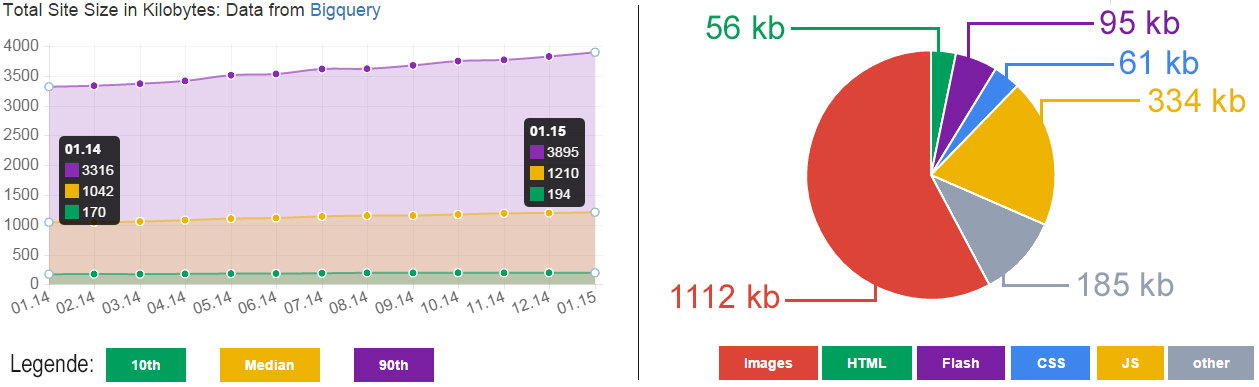
\includegraphics[width=\textwidth]{site_weight2.jpg}
				\caption{Seitenanalyse der populärsten Seiten des Webs (Eigene Abbildung - Daten via \url{bigqueri.es}: Gesamte Auswertung \url{http://tinyurl.com/o8vawxd} )}
				\label{fig:site_weight}
			\end{center}
		\end{figure}

		\subsubsection{Progressive Image Rendering} % (fold)
		\label{ssub:progressive_image_rendering}
			Eigentlich eine sehr alte Technik ist das "`Progressive Image Rendering"'. Es kam längere Zeit außer Mode Bilder als Progressive zu speichern. Der Trend hat sich nun aber wieder geändert und Progressive Images gilt als "`Best Practice"' im Web. Sowohl Webpagetest als auch Google schlagen vor, Bilder Progressive an den Anwender auszuliefern. Testet man eine Seite via Webpagetest.org, so bekommt man unter dem Reiter "`Compress Images"' beispielsweise solch eine Auswertung:
			\begin{quote}
				Use Progressive JPEGs: 100/100\\
				124.8 KB of a possible 124.8 KB (100\%) were from progressive JPEG images
			\end{quote}

			Abbildung \ref{fig:progressive_images} zeigt einmal den normalen Ladevorgang eines Bildes (unten) gegenüber dem "`Progressive Rendering"' (oben).

			\begin{figure}[htbp]
				\begin{center}
					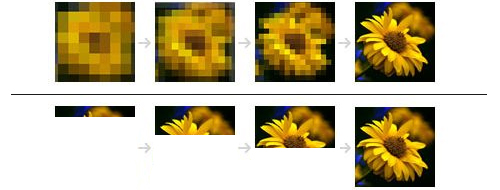
\includegraphics[width=0.7\textwidth]{progressive_images.jpg}
					\caption{Progressives Bilder laden}
					\label{fig:progressive_images}
				\end{center}
			\end{figure}

			Nicht nur sind Progressive Images fast immer ein paar Kilobyte kleiner, sie erhöhen auch die \texttt{Perceived Performance} für den Anwender. Wo bei normalen Bildern lange Zeit eine weiße Lücke klafft, ist bei Progressive Images bereits sehr viel früher das volle Bild zu sehen. Das PNG Äquivalent für Progressive-Jpeg's ist "`Interlaced"'. Bilder sollten zum Beispiel in Photoshop über den Reiter: Datei -> für Web speichern... entweder Progressive oder als Interlaced gespeichert werden.
		% subsubsection progressive_image_rendering (end)

		\subsubsection{Image Spriting} % (fold)
		\label{ssub:image_spriting}
			"`Image Spriting"' bezeichnet das Kombinieren von vielen kleinen Bilddateien zu einer einzigen großen Datei.  Mittels CSS lässt sich aus dem Bild dann das Gewünschte Icon auswählen.

			\begin{figure}[htbp]
				\begin{center}
					
\includegraphics[width=0.6\textwidth]{image_sprites.jpg}
					\caption{Image Sprite von verschiedenen Icons}
					\label{fig:image_sprites}
				\end{center}
			\end{figure}
			
			Der Vorteil dieser Methode ist, dass nur ein Request benötigt wird um alle Icons, die für die Seite benötigt werden, herunterzuladen. Der Nachteil ist, dass durch die größere Datei der Download länger dauern kann und sich so die Zeit für das erste Rendern verringert. Auch bei einer einzigen Änderung, muss die ganze Datei (die im besten Fall bereits gecached wurde) neu heruntergeladen werden.
			
		% subsubsection image_spriting (end)


		\subsubsection{Bild Komprimierung} % (fold)
		\label{ssub:bild_komprimierung}
			Bei der Komprimierung von Bildern unterscheidet man zwischen zwei Arten: "`Lossless"' und "`Lossly"'.
			\begin{itemize}
				\item Lossless bezeichnet die Komprimierung eines Bildes, ohne dabei die Qualität des Bildes zu verändern. So werden bei Lossless zum Beispiel die Metadaten eines Bildes entfernt, die von einer Kamera bei der Aufnahme hinzugefügt werden.
				\item Lossly ist die reduzierung der Bildgröße auf kosten von Qualität. Für die meisten Bilder ist diese Reduzierung aber durchaus Legetim und oftmals sind die Einbußen mit bloßem Auge nicht zu erkennen. Lossly Komprimierung kann aber durchaus bis zu rund 40\% der Bildgröße reduzieren.
			\end{itemize}

			Google hat ein eigenes Bildformat namens "`Webp"' entwickelt und soll bis zu 30\% der Bildgröße bei gleichbleibender Qualität einsparen. Allerdings ist dieses Format nur im Chrome Browser und Opera (der auf Chrome basiert) unterstützt.\autocite{canIuse}

			Eine bessere Alternative ist moz-jpeg. Das ist ein von Mozilla entwickelter JPEG Bild Encoder um die Bildgröße ohne Qualitätseinbußen zu verringern. Dabei bleibt das .jpg Format erhalten und ist somit überall einsetzbar.

			\begin{quote}
				\textit{"`For the short term Mozilla has developed MozJPEG — a modernized JPEG encoder that offers better compression while remaining fully standard-compliant, so it’s compatible with all browsers, operating systems and native apps, and you can use it today without waiting for the whole world to upgrade"'\autocite{mozJPEG}}
			\end{quote}

			Allerdings ist die Verwendung nicht ganz so einfach wie in diesem Zitat dargestellt und es ist das eigenständige Compilieren von \texttt{C}-Code\footnote{Das Repository ist hier zu finden: \url{https://github.com/mozilla/mozjpeg} und eine Anleitung gibt es hier: \url{http://calendar.perfplanet.com/2014/mozjpeg-3-0/}} nötig, um dies auf dem eigenen Betriebssystem zu verwenden.\\
			Glücklicherweise es gibt eine Webanwendung\footnote{Webanwendung zur Verwendung von moz jpeg: \url{https://imageoptim.com/mozjpeg}} mit der ganz einfach per "`drag and drop"' Bilder mittels diesem Encoder komprimiert werden können. Je nach Bild lassen sich so mehrere Hundert Kilobyte einsparen (abhängig von der Qualitätseinstellung und größe des Bildes).\\

			Natürlich bietet auch Photoshop oder IrfanView (Kostenlos) umfangreiche möglichkeiten die Größe von Bildern zu verringern. Moz-jpeg schafft dies allerdings mit einem qualitativ besseren Ergebnis bei zudem kleinerer Bildgröße. Eine Verwendung sollte auf jedenfall in betracht gezogen werden.

		% subsubsection bild_komprimierung (end)

		\subsubsection{Responsive Images} % (fold)
		\label{ssub:responsive_images}
			"`Responsive Images"' ist eine auf das Gerät des Endanwenders angepasste Auslieferung von Bildern. Auf vielen Webanwendungen sieht man folgendes:

			\begin{figure}[htbp]
				\begin{center}
					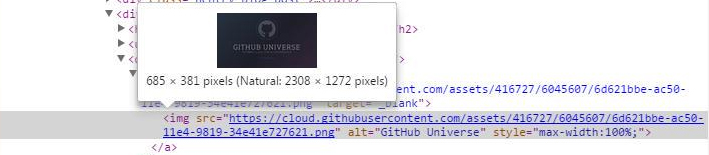
\includegraphics[width=\textwidth]{downsampling.jpg}
					\caption{Downsampling auf GitHub (Eigene Abbildung via Chrome Developer Tool)}
					\label{fig:downsampling}
				\end{center}
			\end{figure}

			Das Bild wurde nicht nur viel zu Groß gewählt, es wird auch auf jedem Gerät, egal ob Tablet, Smartphone oder Desktop die selbe Anzahl an Bytes über die Leitung gesendet. Diese Methode nennt man Downsampling. Das bedeutet, dass nicht das Bild selbst verkleinert wird, sondern der Browser das Bild herunterläd und dann auf die entsprechende Größe skaliert. Das kostet nicht nur Rechenleistung sondern vor allem sehr viel unnötige Bandbreite und sollte unter allen Umständen vermieden werden.\\

			Seit HTML 5 gibt es ein neues HTML Attribut namens \texttt{srcset}. Dieses Attribut ist leider noch nicht in allen Browsern implementiert, hat aber immerhin bereits eine Globale Abdeckung von rund 50\% \autocite{canIuse}. Für dieses Problem gibt es allerdings abhilfe. Es gibt ein Polyfill \footnote{\textit{"`Ein Polyfill [...] ist ein - meist in Javascript geschriebender - Code-Baustein, der in älteren Browsern eine neuere, von diesen nicht unterstützte Funktion mittels eines Workarounds nachrüsten soll. Beispielsweise sind Features von HTML5 in älteren Browsern nicht verfügbar. Webseiten können diese Funktionen trotzdem verwenden, wenn sie ein entsprechendes Polyfill mitliefern."'}\autocite{wikipediaPolyfill}} namens "`Picturefill"'\footnote{Das offizielle Picturefill Projekt ist hier zu finden: \url{http://scottjehl.github.io/picturefill/}}, dass genau diese Funktionalität für alle Browser zur Verfügung stellen kann. Nötig ist dazu nur das herunterladen und Einbinden des Skripts in das HTML Dokument. Dadurch wird folgendes Listing möglich: 

			\begin{lstlisting}[captionpos=b, caption=Srcset in Verwendung, label=lst:srcset]
			<picture id="hero-image">
		    <source srcset="someImg_lg.jpg" media="(min-width: 1367px)">
		    <source srcset="someImg_md.jpg" media="(min-width: 768px)">
		    <source srcset="someImg_xs.jpg" media="(min-width: 300px)">
		    <img srcset="fallback_md.jpg" alt="Some alt text">
			</picture>
			\end{lstlisting}

			Das bedeutet, dass Smartphones mit einer Breite von > 300px < 768px das Bild "`someImg\_xs"' bekommen. Tablets mit 768px < 1367px bekommen das mittlere Bild und alles was über 1367px ist bekommen die größte Version zu Verfügung gestellt. Falls der Anwender Javascript im Browser deaktiviert, ist es möglich ein \texttt{fallback}-Bild zu setzen (Listing: Zeile 8). Man kann sogar einen Schritt weiter gehen und auch das Bildformat auf entsprechend dem Aufrufenden Gerät anpassen:

			\begin{lstlisting}[captionpos=b, caption=Srcset mit webp, label=lst:srcsetWebp]
			<picture id="hero-image">
		    <source srcset="someImg_lg.webp" type="image/webp" media="(min-width: 1367px)">
		    <source srcset="someImg_lg.jpg" media="(min-width: 1367px)">
		    <source srcset="someImg_md.webp" type="image/webp" media="(min-width: 768px)">
		    <source srcset="someImg_md.jpg" media="(min-width: 768px)">
		    <source srcset="someImg_xs.webp" type="image/webp" media="(min-width: 300px)">
		    <source srcset="someImg_xs.jpg" media="(min-width: 300px)">
		    <img srcset="fallback_md.jpg" alt="Some alt text">
			</picture>
			\end{lstlisting}

			Wie zu sehen ist wurden 3 Zeilen eingefügt, die sich lediglich im Typ unterscheiden. Das bedeutet, dass Anwender mit Chrome Browser das Chrome eigene Bildformat .webp bekommen und alle anderen das normale .jpg Format. Voraussetzung ist natürlich, all diese Bilder in ihren verschiedenen Auflösungen und Formaten anzulegen und bereit zu stellen, was einen Mehraufwand bedeutet.
			Picturefill ermöglicht es, Downsampling zu vermeiden und einen auf das Gerät angepasste Version des Bildes auszuliefern. Dadurch sinkt die Anzahl von Bytes die Übertragen werden müssen enorm.

		% subsubsection responsive_images (end)

		\subsubsection{Adaptive Images} % (fold)
		\label{ssub:adaptive_images}
			Adaptive Images ist ein PHP-Skript\footnote{Mehr über dieses Skript ist hier zu finden: \url{http://adaptive-images.com/}}, das mit Hilfe einer htaccess Datei Bilder auf dem Server automatisch auf die verschiedenen Gerätegrößen zuschneidet. Ruft ein Anwender die Seite auf, prüft das Skript die Größe des Bildschirms und liefer anschlißend das für ihn passende Bild aus. 

		% subsubsection adaptive_images (end)

		\subsubsection{Verzögertes Laden von Bildern} % (fold)
		\label{ssub:verzögertes_laden_von_bildern}
			
		% subsubsection verzögertes_laden_von_bildern (end)

	% subsection bilder_optimieren (end)

	\subsection{Prozess der Validierung}
	\label{sub:prozess_der_validierung}
		Bereits zu Beginn des Projekts war es wichtig es messbar zu machen. Dafür wurde eine Testumgebung aufgebaut, mit deren Hilfe die Seite nach ihrer Geschwindigkeit getestet werden kann. Ganz entscheidend war dabei die Webpagetest API in Verbindung mit Google Spreadsheets. Damit ließen sich die Tests automatisiert regelmäßig ausführen und die Daten wurden automatisch in einer Tabelle gespeichert. Die volle Sammlung der Daten über den Zeitraum der Arbeit hinweig ist hier zu finden: \url{http://tinyurl.com/l5usz79}. Diese Daten wurden in Diagrammen aufbereitet und sind unter: \url{http://bithugger.github.io/bachelorthesis/} zu finden.

	1089 Testläufe über Webpagtest: Zeiraum: 1 Monat

	\begin{figure}[htbp]
		\begin{center}
			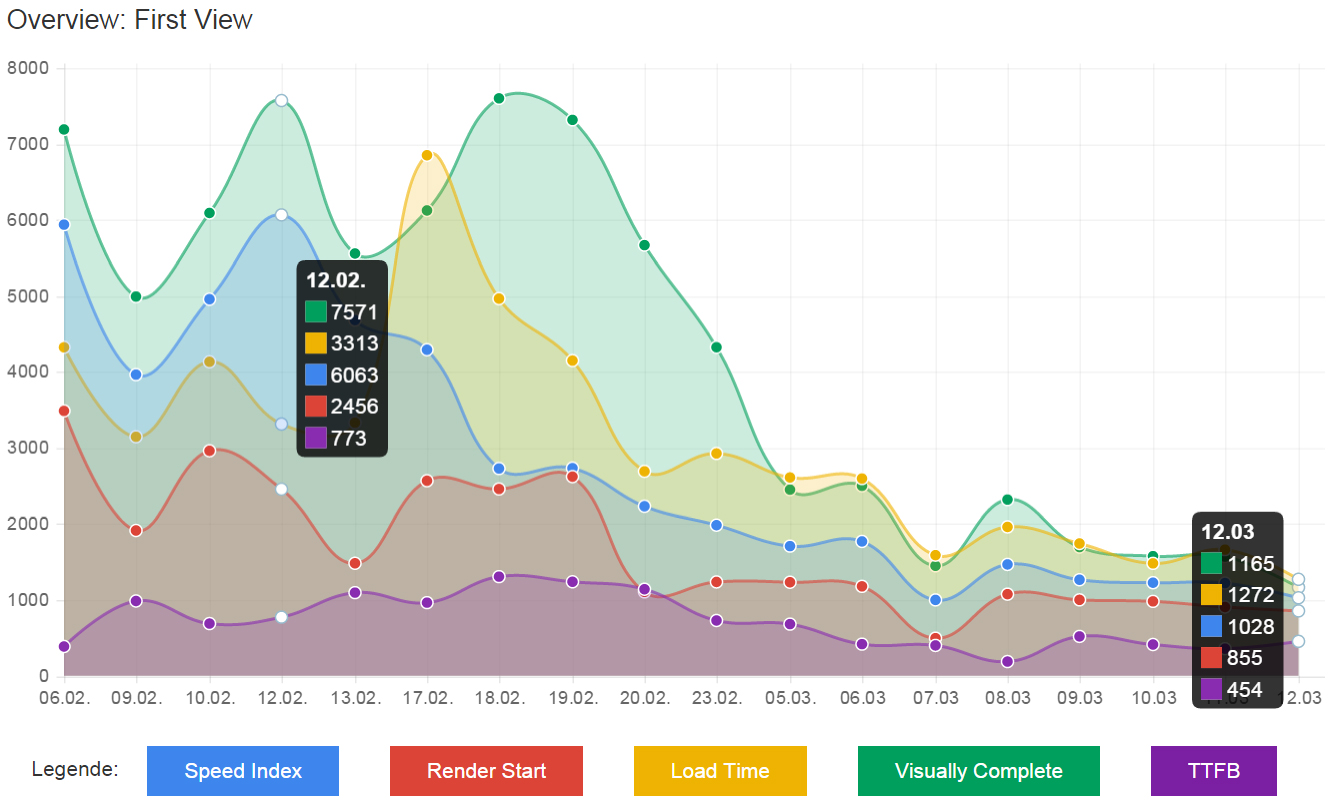
\includegraphics[width=\textwidth]{data_all.jpg}
			\caption{...}
			\label{fig:data_all}
		\end{center}
	\end{figure}
	
	todo
	
	% subsection prozess_der_validierung (end)

	

% section entwicklung (end)